In this section, the explanation will only focus on the particles and energy range that are interesting for this thesis, which are electrons ($0-18~\keV$) and photons in the visible range.

On the one hand, electrons have charge so their interaction with matter are mainly produced with the orbital electrons that there are in that matter, due to the Coulomb force. The trajectory which electrons follow is much more tortuous than other heavier particles because the mass of the interacting particles is equal, electrons. Furthermore, for the same reason, these electrons lost a significant amount of energy in each collision.

In order to speak about the total energy lost of particles in matter the specific energy loss is defined as $S=-\frac{dE}{dx}$ which expresses the energy loss suffered by the particle per unit of trajectory. In the case of electrons, this total energy loss has two main contributions, the collisions (elastic and inelastic) and radiative processes (bremsstrahlung):

$$\frac{dE}{dx} \approx \left(\frac{dE}{dx}\right)_{c} + \left(\frac{dE}{dx}\right)_{br} ~\cite{Knoll} \cite{Leo} \qquad  \frac{\left(\frac{dE}{dx}\right)_{br}}{\left(\frac{dE}{dx}\right)_{c}} \approx \frac{EZ}{700} ~\cite{Knoll}$$

Where $E$ is the energy of the electron in $\MeV$ and $Z$ is the atomic number of the absorbing material. Due to this energy loss, the electrons can only penetrate a material as far as they go before losing their total energy. This distance is known as range and, in the case of tritium electrons, its value is seen in the table \ref{MeanFreePathTritium}.

On the other hand, photons don't have charge. Its possible interactions with the matter are photoelectric effect, Compton effect, coherent scattering and pair production and the probability of each process depends on the energy of the photon, $E_\gamma = h\nu$, and the atomic number of the material, Z, as you can see in the figure \ref{ProcessesPhotons}.

\begin{figure}[htbp]
\centering
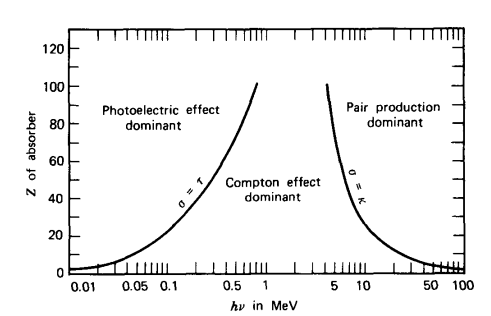
\includegraphics[scale=0.75]{3DesignPrinciples/DominantProcessesPhotons.png}
\caption{Domain regions of the three most probable types of interactions of gamma rays with matter. The lines show the values of Z and $h\nu$ where the two neighboring effects are equally likely.\label{ProcessesPhotons}~\cite{Knoll}~\cite{Leo}}
\end{figure}

We have to take into account that the only relevant photons for this thesis are in the visible range, between $400$ and $700~\nano\meter$, that corresponds with energies of the order of the $\eV$. Therefore the last effect, pair productions, will be not explained here because it needs a photon energy equal or more than $1.022~\MeV$ for happening and it is not our case.

The photoelectric effect occurs when a photon interacts with an orbital electron in the material, losing all its energy. This energy is absorbed by the electron that is released from the atom (ionization). The energy of the resulting electron is:

$$E_e = E_\gamma - E_b ~\cite{Knoll}\cite{Leo}$$

Where $E_e$ is the energy of the electron released and $E_b$ is the binding energy of the electron in this material. The probability of this effect depends on the number of available electrons through the variable Z, and the energy of the electron according to the following expression:

$$\left(Pr\right)_{Ph-eff} \approx \frac{Z^n}{E_\gamma^{3.5}}~\cite{Knoll}$$

As we can see in this expression and in the figure \ref{ProcessesPhotons}, the photoelectric effect is most probably if we use elements with high atomic number. This is the reason why elements with high atomic number are the best isulators against gamma radiation and this is the reason why we use lead ($Z=82$) for building our passive shielding as we will see in the section \ref{sec:PasiveShields}. 

The Compton effect occurs when the photon interacts with an orbital electron of the material, transferring part of this energy to the electron, which is released, and this photon is scattered at an angle $\theta$ with respect to the original direction. If we neglect the binding energy, the energy transfered to this electron, $E_e$, is shown in the following equation:

$$E_e=\frac{\frac{E_\gamma^2}{m_oc^2}\left(1-cos\theta\right)}{1+ \frac{E_\gamma^2}{m_oc^2}\left(1-cos\theta\right)}~\cite{Knoll}\cite{Leo}$$

Where $m_0$ is the rest mass of the electron and $c$ is the speed of the light in the vacumm. The probability of the Compton effect is proporcional to the atomic number(more available electrons), Z,  and decreases with the energy of the photon. 

As we can see in the figure \ref{ProcessesPhotons}, in the energies of the photons belonging to the visible range of the electromagnetic spectrum (of the order of eV), the Compton effect is only more likely in very light materials, (Z<4). For heavier materials the photoelectric effect is the dominant effect. This is the reason why we use elements with high number atomic in the cathode of the our PMTs.

Finally, in the coherent scattering, the atom is neither excitation nor ionization and the photon conserve all their energy in this collision. This effect is more probably for photons with low energies and materials with high atomic numbers.

Because of the fact that the energy of the photon doesn't change we will not speak more about this effect but it is important since this effect change de direction of photons and it will affect to their mean free path.